% CSC302 lecture slides adapted from Heather Macbeth, The Mechanics of Proof.
\documentclass[aspectratio=169,11pt]{beamer}
\usepackage[T1]{fontenc}
\usepackage{lmodern}
\usepackage{amsmath,amssymb,mathtools}
\usepackage{booktabs,array,listings,tikz}
\usetikzlibrary{arrows.meta,positioning,calc}
\definecolor{ProofNavy}{HTML}{18324F}
\definecolor{ProofTeal}{HTML}{007D82}
\definecolor{ProofPaper}{HTML}{F3F6F8}
\usetheme{default}
\setbeamercolor{normal text}{fg=ProofNavy,bg=white}
\setbeamercolor{structure}{fg=ProofTeal}
\setbeamercolor{frametitle}{fg=ProofNavy}
\setbeamercolor{block title}{fg=white,bg=ProofNavy}
\setbeamercolor{block body}{fg=ProofNavy,bg=ProofPaper}
\setbeamercolor{block title example}{fg=white,bg=ProofTeal}
\setbeamercolor{block body example}{fg=ProofNavy,bg=ProofPaper}
\setbeamerfont{frametitle}{size=\Large,series=\bfseries}
\setbeamertemplate{navigation symbols}{}
\setbeamertemplate{itemize item}{\small\textbullet}
\setbeamertemplate{footline}{%
  \leavevmode\hbox{%
  \begin{beamercolorbox}[wd=.86\paperwidth,ht=2.8ex,dp=1.2ex,leftskip=1.6em]{author in head/foot}%
    \scriptsize CSC302\quad\textbar\quad\insertshorttitle
  \end{beamercolorbox}%
  \begin{beamercolorbox}[wd=.14\paperwidth,ht=2.8ex,dp=1.2ex,rightskip=1.6em plus1fil]{date in head/foot}%
    \scriptsize\insertframenumber/\inserttotalframenumber
  \end{beamercolorbox}}}
\setbeamersize{text margin left=8mm,text margin right=8mm}
\lstdefinelanguage{Lean}{%
  morekeywords={example,theorem,lemma,def,by,calc,have,exact,apply,intro,intros,constructor,rcases,rfl,rw,ring,numbers,linarith,nlinarith,rel,extra,addarith,obtain,left,right,use,choose,dsimp,change,ext,fun,show,from,at,with,induction,case,decide,contradiction,push_neg,by_cases,by_contra,assumption,existsi,simp,simpa},
  sensitive=true,morecomment=[l]{--},morestring=[b]"}
\lstset{language=Lean,basicstyle=\ttfamily\small,keywordstyle=\color{ProofTeal}\bfseries,
  commentstyle=\color{gray},stringstyle=\color{ProofNavy},showstringspaces=false,
  columns=fullflexible,keepspaces=true,breaklines=true,frame=single,
  rulecolor=\color{ProofTeal!30},backgroundcolor=\color{ProofPaper},
  aboveskip=0.5em,belowskip=0.4em}
\newcommand{\N}{\mathbb{N}}
\newcommand{\Z}{\mathbb{Z}}
\newcommand{\Q}{\mathbb{Q}}
\newcommand{\R}{\mathbb{R}}
\newcommand{\coursechapter}[2]{%
  \title[Chapter #1: #2]{Chapter #1\\#2}%
  \subtitle{The Mechanics of Proof \textbar{} CSC302 lecture notes}%
  \author{Based on Heather Macbeth's textbook}%
  \date{}%
}
\newcommand{\sourcecredit}[1]{\par\vfill{\tiny Source: Heather Macbeth, \emph{The Mechanics of Proof}, #1.}}
\newcommand{\bookurl}{\url{https://hrmacbeth.github.io/math2001/}}
\hypersetup{colorlinks=true,urlcolor=ProofTeal,linkcolor=ProofNavy}

\coursechapter{6}{Induction}
\begin{document}
\begin{frame}
  \titlepage
\end{frame}

% Source: Chapter 6, complete published HTML and all seven companion Lean files.
% Pinned source commit: e660f42b13ddcb6d12b52ba036d6bd071a0cfb9b.
% Original instructional prose, layouts, and diagram; mathematical statements follow cited sources.
% Listings are teaching material for the source's Lean 4.3 / math2001_init environment.
% No Lean compilation is claimed. Historical termination_by syntax is intentional.

\section{6.1 Introduction}
% Source: Section 6.1, Example 6.1.1.
\begin{frame}{6.1 Induction: an infinite chain of implications}
For a proposition $Q(n)$ indexed by $n\in\N=\{0,1,2,\ldots\}$, prove
\[
 Q(0),\qquad \forall k\in\N,\quad Q(k)\Longrightarrow Q(k+1).
\]
These two facts establish $Q(n)$ for every natural number $n$.
\begin{block}{Worked example: $2^n\ge n+1$ for every $n\in\N$}
Base: $2^0=1=0+1$. Fix $k\in\N$ and assume $2^k\ge k+1$.
Then
\[
 2^{k+1}=2\cdot2^k\ge2(k+1)=(k+2)+k\ge k+2.
\]
The last inequality uses $k\ge0$; the first uses the hypothesis at $k$.
\end{block}
The induction hypothesis is available at $k$, while the goal concerns $k+1$.
\sourcecredit{Section 6.1, Example 6.1.1}
\end{frame}

% Source: Example 6.1.1; original numerical variant and proof organization.
\begin{frame}[fragile]{Lean: identify the base and successor goals}
Here is a closely related claim, $n+1\le3^n$, over $\N$.
\begin{lstlisting}
example (n : Nat) : n + 1 <= 3 ^ n := by
  simple_induction n with k IH
  . numbers
  . calc
      k + 1 + 1 <= 3 * (k + 1) := by addarith
      _ <= 3 * 3 ^ k := by rel [IH]
      _ = 3 ^ (k + 1) := by ring
\end{lstlisting}
\begin{itemize}
\item \texttt{simple\_induction} gives the base goal and a successor goal with \texttt{IH}.
\item \texttt{rel [IH]} transports an inequality through multiplication by $3$.
\item \texttt{addarith} handles linear arithmetic; \texttt{ring} handles the identity.
\end{itemize}
\sourcecredit{Section 6.1, Example 6.1.1}
\end{frame}

% Source: Example 6.1.3; supplies the induction promised in Chapter 3.
% Original witness-based proof, valid for every integer modulus including zero.
\begin{frame}{Powers preserve congruence: prove the general rule}
Let $a,b,m\in\Z$ with $a\equiv b\pmod m$. We prove
$a^n\equiv b^n\pmod m$ for every $n\in\N$.
Choose $v\in\Z$ with $a-b=mv$.

\textbf{Base:} $a^0-b^0=1-1=m\cdot0$.

\textbf{Step:} fix $k\in\N$ and assume $a^k-b^k=mu$ for some $u\in\Z$.
Then
\[
\begin{aligned}
 a^{k+1}-b^{k+1}
 &=a(a^k-b^k)+b^k(a-b)\\
 &=a(mu)+b^k(mv)\\
 &=m(au+b^kv).
\end{aligned}
\]
The new witness $au+b^kv$ is an integer. Induction completes the proof.
No division by $m$ is used, so the argument also covers $m=0$.
\sourcecredit{Section 6.1, Example 6.1.3; general rule used in Chapter 3}
\end{frame}

% Source: Examples 6.1.5--6.1.6.
\begin{frame}[fragile]{Starting at a threshold}
``For all sufficiently large $n$'' means
\[
 \exists N\in\N\;\forall n\in\N,\quad N\le n\Longrightarrow Q(n).
\]
For $Q(n): 2^n\ge n^2$, choose $N=4$. The base is $16=4^2$.
For $k\ge4$, assume $2^k\ge k^2$. Since
\[
 2k^2-(k+1)^2=k(k-2)-1\ge4\cdot2-1=7,
\]
we get $2^{k+1}\ge2k^2\ge(k+1)^2$.

\textbf{Lean setup pattern} for a goal with \texttt{hn : 4 <= n}:
\begin{lstlisting}
induction_from_starting_point n, hn with k hk IH
\end{lstlisting}
The step now includes \texttt{hk : 4 <= k}; the base is at $4$, not $0$.
\sourcecredit{Section 6.1, Examples 6.1.5--6.1.6}
\end{frame}

% Source: Section 6.1.7, exercise on powers of 5 modulo 8.
\begin{frame}{Practice 6.1: a disjunctive invariant}
Prove, for every $n\in\N$,
\[
 5^n\equiv1\pmod8\quad\text{or}\quad5^n\equiv5\pmod8.
\]
All powers and congruences here are interpreted in $\Z$.
\begin{enumerate}
\item State the base case at $n=0$.
\item Write the exact induction hypothesis at $k$.
\item Split that hypothesis into two cases. Which alternative follows at $k+1$?
\end{enumerate}
In Lean, a disjunctive hypothesis can be split using
\texttt{obtain h1 | h5 := IH}; choose the goal's alternative using
\texttt{left} or \texttt{right}.
\sourcecredit{Section 6.1.7}
\end{frame}

% Source: Section 6.1.7; original solution exposition.
\begin{frame}{Solution 6.1: multiplication swaps the alternatives}
Base: $5^0=1$, so choose the first alternative.

Fix $k\in\N$ and assume $5^k\equiv1$ or $5^k\equiv5\pmod8$.
\begin{itemize}
\item If $5^k\equiv1$, then
\[
 5^{k+1}=5\cdot5^k\equiv5\cdot1=5\pmod8.
\]
\item If $5^k\equiv5$, then
\[
 5^{k+1}=5\cdot5^k\equiv25\equiv1\pmod8,
\]
since $25-1=8\cdot3$.
\end{itemize}
Thus the same disjunction holds at $k+1$. Induction completes the proof.
\sourcecredit{Section 6.1.7}
\end{frame}

\section{6.2 Recurrence relations}
% Source: Example 6.2.1.
\begin{frame}{6.2 Recursion defines; induction proves}
A sequence with values in a set $S$ is a function $\N\to S$.
A recurrence specifies initial values and rules for later values.

For example, define $b:\N\to\Z$ by
\[
 b_0=3,\qquad b_{n+1}=b_n^2-2\quad(n\in\N).
\]
Its first terms are $3,7,47,2207$. Each call uses $n<n+1$.
\begin{block}{Invariant: every $b_n$ is odd}
Base: $b_0=2\cdot1+1$.
For $k\in\N$, assume $b_k=2t+1$ for some $t\in\Z$. Then
\[
 b_{k+1}=(2t+1)^2-2=2(2t^2+2t-1)+1.
\]
The displayed integer $2t^2+2t-1$ is the new oddness witness.
\end{block}
\sourcecredit{Section 6.2, Example 6.2.1}
\end{frame}

% Source: Examples 6.2.2--6.2.3; original code uses a shifted invariant.
\begin{frame}[fragile]{A closed formula from a shifted recurrence}
Let $x_0=5$ and $x_{n+1}=2x_n-1$, with $x:\N\to\Z$.
Subtract the fixed point $1$: $x_{n+1}-1=2(x_n-1)$.
\begin{lstlisting}
def x : Nat -> Int
  | 0 => 5
  | k + 1 => 2 * x k - 1

example (n : Nat) : x n - 1 = 4 * 2 ^ n := by
  simple_induction n with k IH
  . rw [x]; numbers
  . calc
      x (k + 1) - 1 = 2 * (x k - 1) := by rw [x]; ring
      _ = 2 * (4 * 2 ^ k) := by rw [IH]
      _ = 4 * 2 ^ (k + 1) := by ring
\end{lstlisting}
Hence $x_n=2^{n+2}+1$, and $x_n\equiv1\pmod4$.
\sourcecredit{Section 6.2, Examples 6.2.2--6.2.3}
\end{frame}

% Source: Example 6.2.4.
\begin{frame}{A recursively defined sum}
Define $A:\N\to\Q$ by $A_0=0$ and
$A_{n+1}=A_n+(n+1)$ for $n\in\N$.
Thus $A_n=1+2+\cdots+n$, with the empty sum equal to $0$.
\begin{block}{Claim: $A_n=\dfrac{n(n+1)}2$ for all $n\in\N$}
Base: $A_0=0=0(0+1)/2$.
For $k\in\N$, assume $A_k=k(k+1)/2$. Then
\[
\begin{aligned}
 A_{k+1}&=A_k+(k+1)\\
 &=\frac{k(k+1)+2(k+1)}2
 =\frac{(k+1)(k+2)}2.
\end{aligned}
\]
\end{block}
Lean connection: \texttt{rw [A]} exposes the recurrence,
\texttt{rw [IH]} replaces the smaller sum, and \texttt{ring} finishes in $\Q$.
\sourcecredit{Section 6.2, Example 6.2.4}
\end{frame}

% Source: Examples 6.2.5--6.2.6; factorial notation corrected throughout.
\begin{frame}{Factorials: keep the divisor universally quantified}
Define $0!=1$ and $(n+1)!=(n+1)n!$ for $n\in\N$.
Induction also gives $n!\ge1$: the base is $1$, and both factors
in $(k+1)k!$ are at least $1$.
\begin{block}{Claim: $\forall n,d\in\N$, $1\le d\le n\Longrightarrow d\mid n!$}
Induct on $n$, keeping the claim about \emph{every} such $d$.
At $n=0$, no $d$ satisfies $1\le d\le0$.

At $n=k+1$, let $1\le d\le k+1$.
\begin{itemize}
\item If $d=k+1$, then $(k+1)!=d\,k!$.
\item Otherwise $d\le k$. The IH gives $k!=dt$ for some $t\in\N$,
so $(k+1)!=d((k+1)t)$.
\end{itemize}
\end{block}
In Lean, introduce $d$ \emph{after} \texttt{simple\_induction n}.
\sourcecredit{Section 6.2, Example 6.2.5}
\end{frame}

% Source: Section 6.2.7, recurrence c; Example 6.2.6.
\begin{frame}{Practice 6.2: formulas and bounds}
\begin{enumerate}
\item Define $c:\N\to\Z$ by
\[
 c_0=7,\qquad c_{n+1}=3c_n-10\quad(n\in\N).
\]
Prove $c_n=2\cdot3^n+5$ for all $n\in\N$.
What fixed point should you subtract from the recurrence?
\item Prove $(n+1)!\ge2^n$ for every $n\in\N$.
Write the successor factorial so that the induction hypothesis applies.
\end{enumerate}
For each proof, name the base case and state the IH before calculating.
\sourcecredit{Section 6.2.7; Example 6.2.6}
\end{frame}

% Source: Section 6.2.7 and Example 6.2.6; original solution exposition.
\begin{frame}{Solution 6.2: expose one recursive layer}
\textbf{1. Closed formula.} The fixed point is $5$, since $3\cdot5-10=5$.
Base: $7=2\cdot3^0+5$.
For $k\in\N$, assuming $c_k=2\cdot3^k+5$ gives
\[
 c_{k+1}=3(2\cdot3^k+5)-10=2\cdot3^{k+1}+5.
\]
\textbf{2. Factorial bound.} Base: $1!=1=2^0$.
For $k\in\N$, assuming $(k+1)!\ge2^k$ gives
\[
 (k+2)!=(k+2)(k+1)!\ge(k+2)2^k\ge2\cdot2^k=2^{k+1}.
\]
The second inequality uses $k+2\ge2$ and $2^k\ge0$.

Both inductions follow the decreasing index in the recursive definition.
\sourcecredit{Section 6.2.7; Example 6.2.6}
\end{frame}

\section{6.3 Two-step induction}
% Source: Example 6.3.1.
\begin{frame}{6.3 Two base cases, two induction hypotheses}
To establish $Q(n)$ for all $n\in\N$, it suffices to prove
\[
 Q(0),\quad Q(1),\quad
 \forall k\in\N,\ (Q(k)\land Q(k+1))\Longrightarrow Q(k+2).
\]
Let $a:\N\to\Z$ satisfy $a_0=2$, $a_1=1$,
$a_{n+2}=a_{n+1}+2a_n$. Claim: $a_n=2^n+(-1)^n$.

\textbf{Bases:} $2=1+1$ and $1=2-1$.
\textbf{Step:} for $k\in\N$, assume the formula at both $k$ and $k+1$.
\[
\begin{aligned}
 a_{k+2}&=(2^{k+1}+(-1)^{k+1})+2(2^k+(-1)^k)\\
 &=4\cdot2^k+(-1)^k=2^{k+2}+(-1)^{k+2}.
\end{aligned}
\]
Both recursive arguments, $k$ and $k+1$, are smaller than $k+2$.
\sourcecredit{Section 6.3, Example 6.3.1}
\end{frame}

% Source: Example 6.3.3; use the source's shifted Fibonacci indexing.
\begin{frame}{Fibonacci: an exponential upper bound}
Define $F:\N\to\Z$ by
\[
 F_0=F_1=1,\qquad F_{n+2}=F_{n+1}+F_n\quad(n\in\N).
\]
The first terms are $1,1,2,3,5,8,13$.
\begin{block}{Claim: $F_n\le2^n$ for all $n\in\N$}
Bases: $F_0=1\le1$ and $F_1=1\le2$.
For $k\in\N$, assume $F_k\le2^k$ and $F_{k+1}\le2^{k+1}$.
Then
\[
 F_{k+2}\le2^{k+1}+2^k=3\cdot2^k
 \le4\cdot2^k=2^{k+2}.
\]
\end{block}
The bound at $k+1$ alone would leave $F_k$ uncontrolled.
\sourcecredit{Section 6.3, Example 6.3.3}
\end{frame}

% Source: Example 6.3.2; original invariant explanation.
\begin{frame}{Sometimes the induction hypothesis needs more information}
For the sequence $a_0=2$, $a_1=1$, $a_{n+2}=a_{n+1}+2a_n$,
prove $a_n\equiv1$ or $5\pmod6$ for $n\ge1$.

Use the stronger assertion that the pair $(a_n,a_{n+1})$ is congruent to
\[
 (1,5)\quad\text{or}\quad(5,1)\pmod6.
\]
Base $n=1$: $(a_1,a_2)=(1,5)$.
For $k\ge1$, assume this assertion at $k$. The recurrence gives
\[
 (1,5)\longmapsto(5,5+2\cdot1)\equiv(5,1),
\]
\[
 (5,1)\longmapsto(1,1+2\cdot5)\equiv(1,5).
\]
Ordinary induction now works on the \emph{pair assertion}; its first component
implies the original claim. This excludes the unwanted pairs $(1,1)$ and $(5,5)$.
\sourcecredit{Section 6.3, Example 6.3.2}
\end{frame}

% Source: Example 6.3.5 and Library/Tactic/Induction.lean.
\begin{frame}[fragile]{Two-step induction from a later starting point}
Define $d:\N\to\Z$ by $d_0=3$, $d_1=1$,
$d_{n+2}=3d_{n+1}+5d_n$.
To prove $d_n\ge4^n$ for $n\ge4$, check \emph{two} bases:
\[
 d_4=267\ge256,\qquad d_5=1096\ge1024.
\]
For $k\ge4$, the hypotheses at $k,k+1$ give
\[
 d_{k+2}\ge3\cdot4^{k+1}+5\cdot4^k
 =17\cdot4^k\ge4^{k+2}.
\]
\textbf{Lean setup patterns:}
\begin{lstlisting}
two_step_induction n with k IH0 IH1
-- Or, with hn : 4 <= n:
two_step_induction_from_starting_point n, hn with k hk IH0 IH1
\end{lstlisting}
Here \texttt{IH0} concerns $k$ and \texttt{IH1} concerns $k+1$.
\sourcecredit{Section 6.3, Example 6.3.5}
\end{frame}

% Source: Section 6.3.6, linear recurrence t.
\begin{frame}{Practice 6.3: a second-order recurrence}
Define $t:\N\to\Z$ by
\[
 t_0=5,\qquad t_1=7,\qquad
 t_{n+2}=2t_{n+1}-t_n\quad(n\in\N).
\]
Prove $t_n=2n+5$ for every $n\in\N$.
\begin{enumerate}
\item Check both bases.
\item State separate hypotheses for $t_k$ and $t_{k+1}$.
\item Substitute both formulas into the recurrence.
\item Explain why checking only $t_0$ cannot determine the whole sequence.
\end{enumerate}
When expressing the formula in Lean, use an integer cast of $n$.
\sourcecredit{Section 6.3.6}
\end{frame}

% Source: Section 6.3.6; original proof and alternate-initial-value illustration.
\begin{frame}{Solution 6.3: the two initial values matter}
Bases: $t_0=5=2\cdot0+5$ and $t_1=7=2\cdot1+5$.

Let $k\in\N$. Assume $t_k=2k+5$ and $t_{k+1}=2(k+1)+5$.
Then
\[
\begin{aligned}
 t_{k+2}&=2\bigl(2(k+1)+5\bigr)-(2k+5)\\
 &=2k+9=2(k+2)+5.
\end{aligned}
\]
The recurrence has the same first difference at each step:
$t_{n+2}-t_{n+1}=t_{n+1}-t_n$.

Changing $t_1$ to $8$ while keeping $t_0=5$ would instead produce
$5,8,11,14,\ldots$. The value at $0$ does not fix the initial difference.
\sourcecredit{Section 6.3.6}
\end{frame}

\section{6.4 Strong induction}
% Source: Examples 6.4.1--6.4.2.
\begin{frame}{6.4 Strong induction: use any smaller input}
For $Q:\N\to\mathrm{Prop}$, prove for every $n\in\N$:
\[
 \bigl(\forall m\in\N,\ m<n\Longrightarrow Q(m)\bigr)
 \Longrightarrow Q(n).
\]
Then $Q(n)$ holds for all $n$. At $n=0$ there are no smaller inputs.
\begin{block}{Worked proof: every $n\ge2$ has a prime divisor}
IH: every $m$ with $2\le m<n$ has a prime divisor.
If $n$ is prime, use $p=n$, since $n=n\cdot1$.
Otherwise, the proper-factor lemma gives $n=mx$ with $2\le m<n$.
The IH gives $m=py$ for a prime $p$, hence $n=p(yx)$.
\end{block}
The least relevant input $n=2$ is prime. The recursive branch uses
$m<n$, which need not be $m=n-1$.
\sourcecredit{Section 6.4, Examples 6.4.1--6.4.2}
\end{frame}

% Source: Example 6.4.1; original recursive proof uses a factored upper bound.
\begin{frame}[fragile]{Lean: a theorem can call itself on smaller inputs}
Using the preceding definition of $F$:
\begin{lstlisting}
theorem fib_upper (n : Nat) : F n <= (2 : Int) ^ n := by
  match n with
  | 0 => rw [F]; numbers
  | 1 => rw [F]; numbers
  | k + 2 =>
      have h0 := fib_upper k
      have h1 := fib_upper (k + 1)
      calc
        F (k + 2) = F (k + 1) + F k := by rw [F]
        _ <= 2 ^ (k + 1) + 2 ^ k := by rel [h0, h1]
        _ = 3 * 2 ^ k := by ring
        _ <= 3 * 2 ^ k + 2 ^ k := by extra
        _ = 2 ^ (k + 2) := by ring
\end{lstlisting}
Both calls decrease the natural-number input. A call at $k+2$ would be circular.
\sourcecredit{Section 6.4, Example 6.4.1}
\end{frame}

% Source: Section 6.4.3, extract_pow_two.
\begin{frame}{Practice 6.4: remove all factors of two}
Show that every $n\in\N$ with $n>0$ admits a representation
\[
 n=2^a x,\qquad a,x\in\N,\qquad x\text{ odd}.
\]
An odd natural number has the form $2u+1$ with $u\in\N$.
\begin{enumerate}
\item What witnesses work when $n$ is odd?
\item If $n=2m$ is positive, prove $0<m<n$ before invoking the IH.
\item Convert a representation of $m$ into one for $n$.
\end{enumerate}
The measure is the positive input $n$; the recursive call is at $m=n/2$.
\sourcecredit{Section 6.4.3}
\end{frame}

% Source: Section 6.4.3; original solution exposition.
\begin{frame}{Solution 6.4: split on parity}
Use strong induction. At a positive $n$, assume the statement for every
$m$ with $0<m<n$.
\begin{itemize}
\item If $n$ is odd, choose $a=0$, $x=n$: $n=2^0n$.
\item If $n$ is even, write $n=2m$. Positivity gives $m\ge1$;
then $m<2m=n$. By the IH, $m=2^a x$ for some odd $x$.
Thus
\[
 n=2m=2\cdot2^a x=2^{a+1}x.
\]
Use witnesses $a+1$ and $x$.
\end{itemize}
At $n=1$ the odd branch closes directly. At $n=0$ the premise $n>0$
is false, so no recursive call or witnesses are required.
\sourcecredit{Section 6.4.3}
\end{frame}

\section{6.5 Pascal's triangle}
% Source: Definition 6.5.1; original dependency diagram, not the textbook figure.
\begin{frame}[fragile]{6.5 Pascal's triangle in two coordinates}
Define $P:\N\times\N\to\N$ by
\[
 P(a,0)=P(0,b)=1,\qquad
 P(a+1,b+1)=P(a+1,b)+P(a,b+1).
\]
\begin{columns}[T]
\begin{column}{.55\textwidth}
\begin{lstlisting}
def pascal : Nat -> Nat -> Nat
  | a, 0 => 1
  | 0, b + 1 => 1
  | a + 1, b + 1 =>
      pascal (a + 1) b + pascal a (b + 1)
termination_by _ a b => a + b
\end{lstlisting}
\end{column}
\begin{column}{.42\textwidth}
\centering
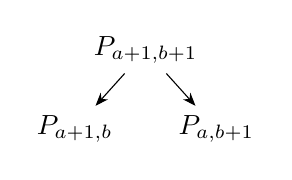
\begin{tikzpicture}[>=Stealth,node distance=9mm]
\node (top) at (0,0) {$P_{a+1,b+1}$};
\node (l) at (-.9,-1) {$P_{a+1,b}$};
\node (r) at (.9,-1) {$P_{a,b+1}$};
\draw[->] (top)--(l); \draw[->] (top)--(r);
\end{tikzpicture}

Each dependency has coordinate sum $a+b+1$, less than $a+b+2$.
\end{column}
\end{columns}
For example: $P(1,1)=2$, $P(1,2)=3$, $P(2,2)=3+3=6$.
\sourcecredit{Section 6.5, Definition 6.5.1}
\end{frame}

% Source: Example 6.5.3, pascal_eq.
% Erratum: the HTML base-case prose drops a!b! and incorrectly equates 1 with (a+b)!.
% The companion Lean statement and base proofs retain both factorial factors.
\begin{frame}{The factorial identity: choose the exact invariant}
For all $a,b\in\N$,
\[
 \boxed{P(a,b)\,a!\,b!=(a+b)!}.
\]
Induct on $a+b$, allowing the IH at \emph{every} pair with smaller sum.
\begin{itemize}
\item If $b=0$, then $P(a,0)a!0!=1\cdot a!\cdot1=(a+0)!$.
\item If $a=0$, then $P(0,b)0!b!=1\cdot1\cdot b!=(0+b)!$.
\end{itemize}
For the interior pair $(a+1,b+1)$, the two needed instances are
\[
 P(a+1,b)(a+1)!b!=(a+b+1)!,
\]
\[
 P(a,b+1)a!(b+1)!=(a+b+1)!.
\]
Each is justified by a decrease of one in the coordinate sum.
\sourcecredit{Section 6.5, Example 6.5.3}
\end{frame}

% Source: Examples 6.5.2--6.5.3; original compressed calculation.
\begin{frame}{The factorial identity: align the two hypotheses}
Write $U=P(a+1,b)$, $V=P(a,b+1)$, and $s=a+b+1$.
The IH says $U(a+1)!b!=s!$ and $Va!(b+1)!=s!$.
Then
\[
\begin{aligned}
 P(a+1,b+1)(a+1)!(b+1)!
 &=(U+V)(a+1)!(b+1)!\\
 &=(b+1)\bigl[U(a+1)!b!\bigr]\\
 &\quad +(a+1)\bigl[Va!(b+1)!\bigr]\\
 &=(b+1)s!+(a+1)s!=(s+1)!.
\end{aligned}
\]
Since $a!b!\ge1$, the identity implies $P(a,b)\le(a+b)!$.
Since factorials are nonzero, division in $\Q$ gives
$P(a,b)=(a+b)!/(a!b!)$.
\sourcecredit{Section 6.5, Examples 6.5.2--6.5.3}
\end{frame}

% Source: Section 6.5.4.
\begin{frame}{Practice 6.5: an edge and a symmetry}
For all natural numbers $a,b$, prove:
\begin{enumerate}
\item $P(a,1)=a+1$, using ordinary induction on $a$.
\item $P(a,b)=P(b,a)$, using induction on $a+b$.
\end{enumerate}
For the symmetry proof, state the IH for arbitrary pairs $(x,y)$ with
$x+y<a+b$. Handle the two boundary directions before the interior.

Lean connection: unfold \texttt{pascal} with \texttt{rw [pascal]}.
For the interior symmetry case, recursively use the symmetry theorem at
$(a+1,b)$ and $(a,b+1)$, then use commutativity of addition.
\sourcecredit{Section 6.5.4}
\end{frame}

% Source: Section 6.5.4; original solution exposition.
\begin{frame}{Solution 6.5: respect both coordinates}
\textbf{Edge.} Base: $P(0,1)=1$. Assume $P(k,1)=k+1$. Then
\[
 P(k+1,1)=P(k+1,0)+P(k,1)=1+(k+1)=k+2.
\]
\textbf{Symmetry.} If either coordinate is zero, both sides are $1$.
For $(a+1,b+1)$, assume symmetry for all smaller sums. Then
\[
\begin{aligned}
 P(a+1,b+1)&=P(a+1,b)+P(a,b+1)\\
 &=P(b,a+1)+P(b+1,a)\\
 &=P(b+1,a)+P(b,a+1)\\
 &=P(b+1,a+1).
\end{aligned}
\]
Both IH calls have sum $a+b+1<a+b+2$.
\sourcecredit{Section 6.5.4}
\end{frame}

\section{6.6 Division Algorithm}
% Source: Definition 6.6.1; table expresses the same ordered branches.
\begin{frame}{6.6 Recursive division on all integers}
Let $M(n,d)=\operatorname{mod}(n,d)$ and
$D(n,d)=\operatorname{div}(n,d)$, both functions $\Z^2\to\Z$.
Use the first applicable row:
\begin{center}
\begin{tabular}{lll}
\toprule
Condition & $M(n,d)$ & $D(n,d)$\\
\midrule
$nd<0$ & $M(n+d,d)$ & $D(n+d,d)-1$\\
$0<d(n-d)$ & $M(n-d,d)$ & $D(n-d,d)+1$\\
$n=d$ & $0$ & $1$\\
otherwise & $n$ & $0$\\
\bottomrule
\end{tabular}
\end{center}
For $d>0$, these respectively address $n<0$, $n>d$, $n=d$, and $0\le n<d$.

The definitions also cover $d\le0$. For example,
$M(n,0)=n$, while $D(0,0)=1$ and $D(n,0)=0$ for $n\ne0$.
\sourcecredit{Section 6.6, Definition 6.6.1}
\end{frame}

% Source: Definition 6.6.1; original proof of the measure decrease using squares.
\begin{frame}{Why recursive division terminates}
Use the nonnegative integer measure $\mu(n,d)=|2n-d|$.
The value of $n$ itself may increase or be negative.
\begin{itemize}
\item If $nd<0$, the call is at $(n+d,d)$. The difference of squared measures is
\[
 (2n+d)^2-(2n-d)^2=8nd<0.
\]
\item If $d(n-d)>0$, the call is at $(n-d,d)$, and
\[
 (2n-3d)^2-(2n-d)^2=-8d(n-d)<0.
\]
\end{itemize}
In both cases, the new absolute value is strictly smaller.
The terminal rows make no calls.

Example: dividing $-7$ by $3$ visits $-7,-4,-1,2$;
the measures are $17,11,5,1$. Thus $M(-7,3)=2$ and $D(-7,3)=-3$.
\sourcecredit{Section 6.6, Definition 6.6.1}
\end{frame}

% Source: Example 6.6.2, fmod_add_fdiv.
% Erratum: its HTML IH repeats (n,d); the quantified smaller-input invariant is at (m,c).
\begin{frame}{Correctness, part I: reconstruct the dividend}
\textbf{Claim:} $M(n,d)+dD(n,d)=n$ for all $n,d\in\Z$.
Induct on $|2n-d|$. The IH is this identity at every $(m,c)$ with
$|2m-c|<|2n-d|$.
\begin{itemize}
\item If $nd<0$, put $M'=M(n+d,d)$ and $D'=D(n+d,d)$.
The IH says $M'+dD'=n+d$, so
\[
 M(n,d)+dD(n,d)=M'+d(D'-1)=(n+d)-d=n.
\]
\item If $d(n-d)>0$, use the IH $M'+dD'=n-d$ at $(n-d,d)$:
\[
 M(n,d)+dD(n,d)=M'+d(D'+1)=(n-d)+d=n.
\]
\item The $n=d$ row gives $0+d\cdot1=n$;
the final row gives $n+d\cdot0=n$.
\end{itemize}
\sourcecredit{Section 6.6, Example 6.6.2}
\end{frame}

% Source: Examples 6.6.3--6.6.4; joint invariant is an original presentation.
\begin{frame}{Correctness, part II: bound the remainder}
\textbf{Claim:} for $n,d\in\Z$ with $d>0$,
\[
 0\le M(n,d)<d.
\]
Induct on $|2n-d|$, with this range statement as the IH at all smaller
inputs with positive divisor.
\begin{itemize}
\item In either recursive row, the divisor stays $d>0$ and the remainder
is unchanged. Apply the IH to $(n+d,d)$ or $(n-d,d)$.
\item If $n=d$, the remainder is $0$, and $0<d$.
\item In the final row, the failed tests give $nd\ge0$ and
$d(n-d)\le0$. Since $d>0$, these imply $0\le n\le d$.
The failed equality test gives $n\ne d$, hence $n<d$.
Here $M(n,d)=n$.
\end{itemize}
The positive-divisor premise is used to cancel $d$ without reversing inequalities.
\sourcecredit{Section 6.6, Examples 6.6.3--6.6.4}
\end{frame}

% Source: Definition 6.6.1 and Examples 6.6.2--6.6.5.
\begin{frame}[fragile]{Lean names and the existence theorem}
The textbook calls $M$ \texttt{fmod} and $D$ \texttt{fdiv}.
These are the relevant lemma applications:
\begin{lstlisting}
-- Context: n d : Int, hd : 0 < d
have hid := fmod_add_fdiv n d
have hlo := fmod_nonneg_of_pos n hd
have hhi := fmod_lt_of_pos n hd
\end{lstlisting}
Together they give witnesses $q=D(n,d)$ and $r=M(n,d)$ for
\[
 \forall n,d\in\Z,\quad d>0\Longrightarrow
 \exists q,r\in\Z,\quad n=r+dq\ \land\ 0\le r<d.
\]
Also $n-r=dq$, so $n\equiv r\pmod d$: every integer has a representative
among $0,1,\ldots,d-1$.

The recursive proofs use \texttt{split\_ifs}, \texttt{cancel}, and the source's
\texttt{termination\_by \_ n d => 2 * n - d}; integer size means absolute value.
\sourcecredit{Section 6.6, Examples 6.6.2--6.6.5}
\end{frame}

% Source: Section 6.6.6, uniqueness exercise; original numerical prompt.
\begin{frame}{Practice 6.6: uniqueness and a negative input}
\begin{enumerate}
\item Follow the recursive definition to compute $M(-8,3)$ and $D(-8,3)$.
Record $|2n-3|$ at each call.
\item Let $n,d,q,q',r,s\in\Z$ with $d>0$ and
\[
 n=r+dq=s+dq',\qquad 0\le r<d,\quad0\le s<d.
\]
Prove $r=s$ and then $q=q'$.
\end{enumerate}
Hint: subtract the reconstruction equations. How large can $r-s$ be?
Which integer multiples of $d$ fit strictly between $-d$ and $d$?
\sourcecredit{Section 6.6.6}
\end{frame}

% Source: Section 6.6.6; original solution and quotient-uniqueness extension.
\begin{frame}{Solution 6.6: a bounded multiple must be zero}
\textbf{Computation:} the inputs are $-8,-5,-2,1$ with divisor $3$.
The measures are $19,13,7,1$. At $1$, the output is $(M,D)=(1,0)$;
three returns subtract $1$ from $D$, giving
\[
 M(-8,3)=1,\qquad D(-8,3)=-3,\qquad -8=1+3(-3).
\]
\textbf{Uniqueness:} subtraction gives $r-s=d(q'-q)$, and the bounds imply
$-d<r-s<d$. Put $t=q'-q\in\Z$.
\begin{itemize}
\item If $t\ge1$, then $dt\ge d$, impossible.
\item If $t\le-1$, then $dt\le-d$, impossible.
\end{itemize}
Thus $t=0$, so $q'=q$ and $r=s$.
The existence theorem plus this argument gives a unique quotient--remainder pair.
\sourcecredit{Section 6.6.6}
\end{frame}

\section{6.7 Euclidean algorithm}
% Source: Definition 6.7.1 and Example 6.7.2.
\begin{frame}{6.7 Euclid's algorithm, including negative inputs}
For $a,b\in\Z$, define $G(a,b)=\gcd(a,b)$ recursively by
\[
 G(a,b)=\begin{cases}
 G(b,M(a,b)),&b>0,\\
 G(b,M(a,-b)),&b<0,\\
 a,&b=0,\ a\ge0,\\
 -a,&b=0,\ a<0.
 \end{cases}
\]
The measure is $|b|$. For $b\ne0$, put $r=M(a,|b|)$.
The remainder theorem gives $0\le r<|b|$, so $|r|<|b|$.

\textbf{Nonnegativity proof:} induct on $|b|$ with IH
$G(x,y)\ge0$ whenever $|y|<|b|$.
If $b=0$, $G(a,0)=|a|\ge0$; otherwise $G(a,b)=G(b,r)\ge0$ by the IH.
In particular, $G(0,0)=0$.
\sourcecredit{Section 6.7, Definition 6.7.1; Example 6.7.2}
\end{frame}

% Source: Example 6.7.3 and companion gcd_dvd_left/gcd_dvd_right.
% Erratum: the HTML IH says nonnegativity; the required invariant is common divisibility.
\begin{frame}{Why the output divides both inputs}
\textbf{Claim:} $G(a,b)\mid a$ and $G(a,b)\mid b$ for all $a,b\in\Z$.
Induct on $|b|$, assuming \emph{both divisibility claims} for all smaller
second-coordinate absolute values.

For $b\ne0$, let $r=M(a,|b|)$, $q=D(a,|b|)$, $g=G(b,r)$.
The IH gives $b=gu$ and $r=gv$ for some $u,v\in\Z$.
\[
 a=\begin{cases}
 r+bq=g(v+uq),&b>0,\\
 r-bq=g(v-uq),&b<0.
 \end{cases}
\]
Thus $g$ divides $a$ as well as $b$, and $g=G(a,b)$.

If $b=0$, $G(a,0)=|a|$: use witness $1$ for $a\ge0$, witness $-1$
for $a<0$, and witness $0$ for divisibility of $b=0$.
\sourcecredit{Section 6.7, Example 6.7.3}
\end{frame}

% Source: Definition 6.7.4; table is original but preserves both sign branches.
\begin{frame}{Extended Euclid: compute coefficients along with the gcd}
Define $L,R:\Z^2\to\Z$ mutually. For $b\ne0$, put
$r=M(a,|b|)$ and $q=D(a,|b|)$.
\begin{center}
\begin{tabular}{lll}
\toprule
Condition & $L(a,b)$ & $R(a,b)$\\
\midrule
$b>0$ & $R(b,r)$ & $L(b,r)-qR(b,r)$\\
$b<0$ & $R(b,r)$ & $L(b,r)+qR(b,r)$\\
$b=0$, $a\ge0$ & $1$ & $0$\\
$b=0$, $a<0$ & $-1$ & $0$\\
\bottomrule
\end{tabular}
\end{center}
Both functions only call the pair $(b,r)$, whose measure $|r|$ is below $|b|$.

The intended invariant is
\[
 L(a,b)a+R(a,b)b=G(a,b).
\]
The change of sign in $R$ matches $a=r+bq$ versus $a=r-bq$.
\sourcecredit{Section 6.7, Definition 6.7.4}
\end{frame}

% Source: Definitions 6.7.1 and 6.7.4; original numerical example (-26,18).
\begin{frame}{Worked computation: descend, then recover coefficients}
For $(a,b)=(-26,18)$, divide with positive divisors:
\[
 -26=10+18(-2),\quad18=8+10(1),\quad
 10=2+8(1),\quad8=0+2(4).
\]
The second inputs have measures $18,10,8,2,0$, so the gcd is $2$.
Recover $(L,R)$ from the last row upward:
\begin{center}
\begin{tabular}{rrrr}
\toprule
$(a,b)$ & $q$ & $L(a,b)$ & $R(a,b)$\\
\midrule
$(2,0)$ & --- & $1$ & $0$\\
$(8,2)$ & $4$ & $0$ & $1$\\
$(10,8)$ & $1$ & $1$ & $-1$\\
$(18,10)$ & $1$ & $-1$ & $2$\\
$(-26,18)$ & $-2$ & $2$ & $3$\\
\bottomrule
\end{tabular}
\end{center}
Check: $2(-26)+3(18)=2$. For example, the last coefficient is
$-1-(-2)\cdot2=3$.
\sourcecredit{Section 6.7, Definition 6.7.4 (numerical variant)}
\end{frame}

% Source: Example 6.7.5, L_mul_add_R_mul.
% Erratum: the HTML IH repeats nonnegativity; use the coefficient identity at smaller pairs.
\begin{frame}{Proving the coefficient identity: positive second input}
\textbf{Theorem:} $L(a,b)a+R(a,b)b=G(a,b)$ for all $a,b\in\Z$.
Induct on $|b|$. The IH is
\[
 L(x,y)x+R(x,y)y=G(x,y)\quad\text{whenever }|y|<|b|.
\]
If $b>0$, let $r=M(a,b)$ and $q=D(a,b)$, so $a=r+bq$.
Write $\ell=L(b,r)$ and $t=R(b,r)$.
The IH gives $\ell b+tr=G(b,r)$. Therefore
\[
\begin{aligned}
 L(a,b)a+R(a,b)b
 &=ta+(\ell-qt)b\\
 &=t(r+bq)+(\ell-qt)b\\
 &=tr+\ell b=G(b,r)=G(a,b).
\end{aligned}
\]
The cancellation of $tbq$ explains the definition of $R(a,b)$.
\sourcecredit{Section 6.7, Example 6.7.5}
\end{frame}

% Source: Example 6.7.5 and matching Lean branches.
% Erratum: for a<0,b=0 the printed calculation has (-1)(-a)=a.
% Correct base: (-1)a+0b=-a=gcd(a,0), as enforced by the Lean definitions.
\begin{frame}{The negative branch and the two terminal cases}
If $b<0$, let $r=M(a,-b)$ and $q=D(a,-b)$.
Now $a=r-bq$. Put $\ell=L(b,r)$ and $t=R(b,r)$.
The IH still says $\ell b+tr=G(b,r)$, since $|r|<|b|$.
\[
\begin{aligned}
 L(a,b)a+R(a,b)b
 &=ta+(\ell+qt)b\\
 &=t(r-bq)+(\ell+qt)b\\
 &=tr+\ell b=G(b,r)=G(a,b).
\end{aligned}
\]
For $b=0$ there is no recursive call:
\[
 \begin{array}{ll}
 a\ge0:&1\cdot a+0\cdot b=a=G(a,0),\\[2pt]
 a<0:&(-1)\cdot a+0\cdot b=-a=G(a,0).
 \end{array}
\]
These cases complete the induction for all integer signs.
\sourcecredit{Section 6.7, Example 6.7.5}
\end{frame}

% Source: Examples 6.7.3--6.7.6; original existential wrapper with explicit refine.
\begin{frame}[fragile]{Lean: mutual recursion and a reusable existence theorem}
The source defines \texttt{L} and \texttt{R} in a \texttt{mutual} block.
Its \texttt{gcd\_dvd\_left} and \texttt{gcd\_dvd\_right} proofs also use
mutual induction. All recursive calls decrease $|b|$.

\textbf{B\'ezout's identity:} for every $a,b\in\Z$, there are $x,y\in\Z$
with $xa+yb=G(a,b)$. Choose $x=L(a,b)$, $y=R(a,b)$.
\begin{lstlisting}
-- In the source's Euclid namespace:
example (a b : Int) :
    Exists (fun x : Int => Exists (fun y : Int =>
      x * a + y * b = gcd a b)) := by
  refine Exists.intro (L a b) ?_
  refine Exists.intro (R a b) ?_
  exact L_mul_add_R_mul a b
\end{lstlisting}
The witnesses need not be unique: replacing $(x,y)$ by
$(x+tb,y-ta)$ for $t\in\Z$ preserves the equation.
\sourcecredit{Section 6.7, Examples 6.7.3--6.7.6}
\end{frame}

% Source: Section 6.7.7; original negative-b computation prompt.
\begin{frame}{Practice 6.7: certify the gcd}
\begin{enumerate}
\item Compute $G(14,-8)$, $L(14,-8)$, and $R(14,-8)$.
Start with $14=6+8\cdot1$. Apply the negative-$b$ branch at the first step.
Verify the resulting linear combination.
\item Let $a,b,d\in\Z$. Prove
\[
 d\mid a\ \land\ d\mid b\quad\Longrightarrow\quad d\mid G(a,b).
\]
Use B\'ezout's identity and divisibility witnesses, without a new induction.
\end{enumerate}
Explain why this property, common divisibility, and nonnegativity characterize
the gcd even when $a$ or $b$ is negative.
\sourcecredit{Section 6.7.7; Definition 6.7.4}
\end{frame}

% Source: Section 6.7.7; original worked solution and zero-case qualification.
\begin{frame}{Solution 6.7: coefficients certify maximality}
\textbf{Computation.} The recursive pairs are
\[
 (14,-8)\to(-8,6)\to(6,4)\to(4,2)\to(2,0).
\]
The quotients (using $|b|$) are $1,-2,1,2$.
Backward coefficient pairs are
\[
 (1,0),\ (0,1),\ (1,-1),\ (-1,-1),\ (-1,-2).
\]
Thus $G(14,-8)=2$ and $(-1)14+(-2)(-8)=2$.

\textbf{Divisibility.} Write $a=du$, $b=dv$ and choose B\'ezout witnesses $x,y$.
Then
\[
 G(a,b)=xa+yb=xdu+ydv=d(xu+yv).
\]
If $(a,b)\ne(0,0)$, the gcd is positive, so every positive common divisor
is at most it. At $(0,0)$ the gcd is $0$; the divisibility characterization
still holds, although there is no largest positive common divisor.
\sourcecredit{Section 6.7.7}
\end{frame}

% References cover all seven source sections, not just the selected examples.
\begin{frame}{References}
Heather Macbeth, \emph{The Mechanics of Proof}, Chapter 6, ``Induction.''
\begin{itemize}
\item Sections 6.1--6.3: introduction, recurrence relations, two-step induction.
\item Sections 6.4--6.5: strong induction and Pascal's triangle.
\item Sections 6.6--6.7: the Division Algorithm and the Euclidean algorithm,
including the extended algorithm and B\'ezout's identity.
\end{itemize}
\href{https://hrmacbeth.github.io/math2001/06_Induction.html}{Published Chapter 6}
\qquad
\href{https://github.com/hrmacbeth/math2001/tree/e660f42b13ddcb6d12b52ba036d6bd071a0cfb9b/Math2001/06_Induction}{Companion Lean source, pinned revision}

Source revision: \texttt{e660f42b13ddc}.

Textbook copyright \textcopyright\ 2022--2024 Heather Macbeth; all rights reserved.
These lecture explanations and diagrams are independently written.
\end{frame}
\end{document}
